% Data-driven paths generated from plotted_grid_acc_nmi.csv.
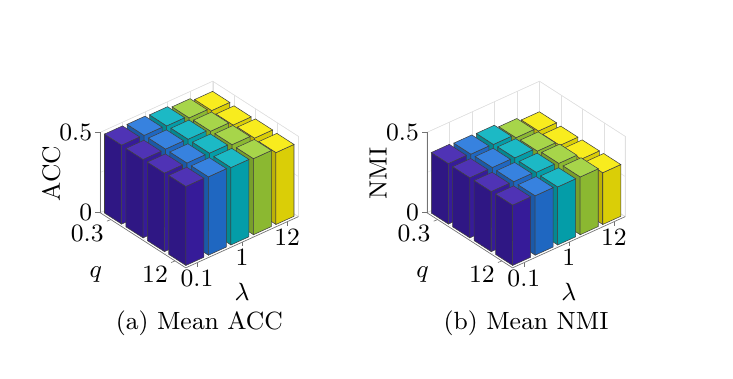
\begin{tikzpicture}[x=1mm,y=1mm,
font=\fontsize{9.2}{10.5}\selectfont,
line join=miter,line cap=butt,
gridline/.style={draw=black!12,line width=0.15pt},
axisline/.style={draw=black!55,line width=0.23pt},
barline/.style={draw=black!75,line width=0.19pt}]
\path[use as bounding box] (0,5.0) rectangle (86,46);
\definecolor{series0}{rgb}{0.24,0.12,0.68}
\definecolor{series1}{rgb}{0.14,0.46,0.86}
\definecolor{series2}{rgb}{0.02,0.7,0.75}
\definecolor{series3}{rgb}{0.62,0.82,0.22}
\definecolor{series4}{rgb}{0.97,0.92,0.03}
\path[fill=white,gridline] (9.200000,22.500000) -- (23.500000,29.000000) -- (23.500000,39.200000) -- (9.200000,32.700000) -- cycle;
\path[fill=white,gridline] (23.500000,29.000000) -- (34.380000,22.000000) -- (34.380000,32.200000) -- (23.500000,39.200000) -- cycle;
\draw[gridline] (9.200000,22.500000) -- (20.080000,15.500000);
\draw[gridline] (9.200000,22.500000) -- (9.200000,32.700000);
\draw[gridline] (12.060000,23.800000) -- (22.940000,16.800000);
\draw[gridline] (12.060000,23.800000) -- (12.060000,34.000000);
\draw[gridline] (14.920000,25.100000) -- (25.800000,18.100000);
\draw[gridline] (14.920000,25.100000) -- (14.920000,35.300000);
\draw[gridline] (17.780000,26.400000) -- (28.660000,19.400000);
\draw[gridline] (17.780000,26.400000) -- (17.780000,36.600000);
\draw[gridline] (20.640000,27.700000) -- (31.520000,20.700000);
\draw[gridline] (20.640000,27.700000) -- (20.640000,37.900000);
\draw[gridline] (23.500000,29.000000) -- (34.380000,22.000000);
\draw[gridline] (23.500000,29.000000) -- (23.500000,39.200000);
\draw[gridline] (9.200000,22.500000) -- (23.500000,29.000000);
\draw[gridline] (23.500000,29.000000) -- (23.500000,39.200000);
\draw[gridline] (11.920000,20.750000) -- (26.220000,27.250000);
\draw[gridline] (26.220000,27.250000) -- (26.220000,37.450000);
\draw[gridline] (14.640000,19.000000) -- (28.940000,25.500000);
\draw[gridline] (28.940000,25.500000) -- (28.940000,35.700000);
\draw[gridline] (17.360000,17.250000) -- (31.660000,23.750000);
\draw[gridline] (31.660000,23.750000) -- (31.660000,33.950000);
\draw[gridline] (20.080000,15.500000) -- (34.380000,22.000000);
\draw[gridline] (34.380000,22.000000) -- (34.380000,32.200000);
\draw[gridline] (9.200000,22.500000) -- (23.500000,29.000000);
\draw[gridline] (23.500000,29.000000) -- (34.380000,22.000000);
\draw[gridline] (9.200000,27.600000) -- (23.500000,34.100000);
\draw[gridline] (23.500000,34.100000) -- (34.380000,27.100000);
\draw[gridline] (9.200000,32.700000) -- (23.500000,39.200000);
\draw[gridline] (23.500000,39.200000) -- (34.380000,32.200000);
\path[barline,fill=series4!76!black] (21.198000,27.655000) -- (23.374000,26.255000) -- (23.374000,35.471732) -- (21.198000,36.871732) -- cycle;
\path[barline,fill=series4!88!black] (23.374000,26.255000) -- (25.662000,27.295000) -- (25.662000,36.511732) -- (23.374000,35.471732) -- cycle;
\path[barline,fill=series4!91!white] (21.198000,36.871732) -- (23.486000,37.911732) -- (25.662000,36.511732) -- (23.374000,35.471732) -- cycle;
\path[barline,fill=series4!76!black] (23.918000,25.905000) -- (26.094000,24.505000) -- (26.094000,33.632268) -- (23.918000,35.032268) -- cycle;
\path[barline,fill=series4!88!black] (26.094000,24.505000) -- (28.382000,25.545000) -- (28.382000,34.672268) -- (26.094000,33.632268) -- cycle;
\path[barline,fill=series4!91!white] (23.918000,35.032268) -- (26.206000,36.072268) -- (28.382000,34.672268) -- (26.094000,33.632268) -- cycle;
\path[barline,fill=series3!76!black] (18.338000,26.355000) -- (20.514000,24.955000) -- (20.514000,34.543231) -- (18.338000,35.943231) -- cycle;
\path[barline,fill=series3!88!black] (20.514000,24.955000) -- (22.802000,25.995000) -- (22.802000,35.583231) -- (20.514000,34.543231) -- cycle;
\path[barline,fill=series3!91!white] (18.338000,35.943231) -- (20.626000,36.983231) -- (22.802000,35.583231) -- (20.514000,34.543231) -- cycle;
\path[barline,fill=series4!76!black] (26.638000,24.155000) -- (28.814000,22.755000) -- (28.814000,31.969293) -- (26.638000,33.369293) -- cycle;
\path[barline,fill=series4!88!black] (28.814000,22.755000) -- (31.102000,23.795000) -- (31.102000,33.009293) -- (28.814000,31.969293) -- cycle;
\path[barline,fill=series4!91!white] (26.638000,33.369293) -- (28.926000,34.409293) -- (31.102000,33.009293) -- (28.814000,31.969293) -- cycle;
\path[barline,fill=series3!76!black] (21.058000,24.605000) -- (23.234000,23.205000) -- (23.234000,32.847960) -- (21.058000,34.247960) -- cycle;
\path[barline,fill=series3!88!black] (23.234000,23.205000) -- (25.522000,24.245000) -- (25.522000,33.887960) -- (23.234000,32.847960) -- cycle;
\path[barline,fill=series3!91!white] (21.058000,34.247960) -- (23.346000,35.287960) -- (25.522000,33.887960) -- (23.234000,32.847960) -- cycle;
\path[barline,fill=series2!76!black] (15.478000,25.055000) -- (17.654000,23.655000) -- (17.654000,33.522580) -- (15.478000,34.922580) -- cycle;
\path[barline,fill=series2!88!black] (17.654000,23.655000) -- (19.942000,24.695000) -- (19.942000,34.562580) -- (17.654000,33.522580) -- cycle;
\path[barline,fill=series2!91!white] (15.478000,34.922580) -- (17.766000,35.962580) -- (19.942000,34.562580) -- (17.654000,33.522580) -- cycle;
\path[barline,fill=series4!76!black] (29.358000,22.405000) -- (31.534000,21.005000) -- (31.534000,30.134301) -- (29.358000,31.534301) -- cycle;
\path[barline,fill=series4!88!black] (31.534000,21.005000) -- (33.822000,22.045000) -- (33.822000,31.174301) -- (31.534000,30.134301) -- cycle;
\path[barline,fill=series4!91!white] (29.358000,31.534301) -- (31.646000,32.574301) -- (33.822000,31.174301) -- (31.534000,30.134301) -- cycle;
\path[barline,fill=series3!76!black] (23.778000,22.855000) -- (25.954000,21.455000) -- (25.954000,31.136610) -- (23.778000,32.536610) -- cycle;
\path[barline,fill=series3!88!black] (25.954000,21.455000) -- (28.242000,22.495000) -- (28.242000,32.176610) -- (25.954000,31.136610) -- cycle;
\path[barline,fill=series3!91!white] (23.778000,32.536610) -- (26.066000,33.576610) -- (28.242000,32.176610) -- (25.954000,31.136610) -- cycle;
\path[barline,fill=series2!76!black] (18.198000,23.305000) -- (20.374000,21.905000) -- (20.374000,31.829906) -- (18.198000,33.229906) -- cycle;
\path[barline,fill=series2!88!black] (20.374000,21.905000) -- (22.662000,22.945000) -- (22.662000,32.869906) -- (20.374000,31.829906) -- cycle;
\path[barline,fill=series2!91!white] (18.198000,33.229906) -- (20.486000,34.269906) -- (22.662000,32.869906) -- (20.374000,31.829906) -- cycle;
\path[barline,fill=series1!76!black] (12.618000,23.755000) -- (14.794000,22.355000) -- (14.794000,32.317062) -- (12.618000,33.717062) -- cycle;
\path[barline,fill=series1!88!black] (14.794000,22.355000) -- (17.082000,23.395000) -- (17.082000,33.357062) -- (14.794000,32.317062) -- cycle;
\path[barline,fill=series1!91!white] (12.618000,33.717062) -- (14.906000,34.757062) -- (17.082000,33.357062) -- (14.794000,32.317062) -- cycle;
\path[barline,fill=series3!76!black] (26.498000,21.105000) -- (28.674000,19.705000) -- (28.674000,29.365443) -- (26.498000,30.765443) -- cycle;
\path[barline,fill=series3!88!black] (28.674000,19.705000) -- (30.962000,20.745000) -- (30.962000,30.405443) -- (28.674000,29.365443) -- cycle;
\path[barline,fill=series3!91!white] (26.498000,30.765443) -- (28.786000,31.805443) -- (30.962000,30.405443) -- (28.674000,29.365443) -- cycle;
\path[barline,fill=series2!76!black] (20.918000,21.555000) -- (23.094000,20.155000) -- (23.094000,30.059060) -- (20.918000,31.459060) -- cycle;
\path[barline,fill=series2!88!black] (23.094000,20.155000) -- (25.382000,21.195000) -- (25.382000,31.099060) -- (23.094000,30.059060) -- cycle;
\path[barline,fill=series2!91!white] (20.918000,31.459060) -- (23.206000,32.499060) -- (25.382000,31.099060) -- (23.094000,30.059060) -- cycle;
\path[barline,fill=series1!76!black] (15.338000,22.005000) -- (17.514000,20.605000) -- (17.514000,30.579948) -- (15.338000,31.979948) -- cycle;
\path[barline,fill=series1!88!black] (17.514000,20.605000) -- (19.802000,21.645000) -- (19.802000,31.619948) -- (17.514000,30.579948) -- cycle;
\path[barline,fill=series1!91!white] (15.338000,31.979948) -- (17.626000,33.019948) -- (19.802000,31.619948) -- (17.514000,30.579948) -- cycle;
\path[barline,fill=series0!76!black] (9.758000,22.455000) -- (11.934000,21.055000) -- (11.934000,31.084547) -- (9.758000,32.484547) -- cycle;
\path[barline,fill=series0!88!black] (11.934000,21.055000) -- (14.222000,22.095000) -- (14.222000,32.124547) -- (11.934000,31.084547) -- cycle;
\path[barline,fill=series0!91!white] (9.758000,32.484547) -- (12.046000,33.524547) -- (14.222000,32.124547) -- (11.934000,31.084547) -- cycle;
\path[barline,fill=series2!76!black] (23.638000,19.805000) -- (25.814000,18.405000) -- (25.814000,28.232612) -- (23.638000,29.632612) -- cycle;
\path[barline,fill=series2!88!black] (25.814000,18.405000) -- (28.102000,19.445000) -- (28.102000,29.272612) -- (25.814000,28.232612) -- cycle;
\path[barline,fill=series2!91!white] (23.638000,29.632612) -- (25.926000,30.672612) -- (28.102000,29.272612) -- (25.814000,28.232612) -- cycle;
\path[barline,fill=series1!76!black] (18.058000,20.255000) -- (20.234000,18.855000) -- (20.234000,28.813017) -- (18.058000,30.213017) -- cycle;
\path[barline,fill=series1!88!black] (20.234000,18.855000) -- (22.522000,19.895000) -- (22.522000,29.853017) -- (20.234000,28.813017) -- cycle;
\path[barline,fill=series1!91!white] (18.058000,30.213017) -- (20.346000,31.253017) -- (22.522000,29.853017) -- (20.234000,28.813017) -- cycle;
\path[barline,fill=series0!76!black] (12.478000,20.705000) -- (14.654000,19.305000) -- (14.654000,29.264858) -- (12.478000,30.664858) -- cycle;
\path[barline,fill=series0!88!black] (14.654000,19.305000) -- (16.942000,20.345000) -- (16.942000,30.304858) -- (14.654000,29.264858) -- cycle;
\path[barline,fill=series0!91!white] (12.478000,30.664858) -- (14.766000,31.704858) -- (16.942000,30.304858) -- (14.654000,29.264858) -- cycle;
\path[barline,fill=series1!76!black] (20.778000,18.505000) -- (22.954000,17.105000) -- (22.954000,27.054789) -- (20.778000,28.454789) -- cycle;
\path[barline,fill=series1!88!black] (22.954000,17.105000) -- (25.242000,18.145000) -- (25.242000,28.094789) -- (22.954000,27.054789) -- cycle;
\path[barline,fill=series1!91!white] (20.778000,28.454789) -- (23.066000,29.494789) -- (25.242000,28.094789) -- (22.954000,27.054789) -- cycle;
\path[barline,fill=series0!76!black] (15.198000,18.955000) -- (17.374000,17.555000) -- (17.374000,27.529757) -- (15.198000,28.929757) -- cycle;
\path[barline,fill=series0!88!black] (17.374000,17.555000) -- (19.662000,18.595000) -- (19.662000,28.569757) -- (17.374000,27.529757) -- cycle;
\path[barline,fill=series0!91!white] (15.198000,28.929757) -- (17.486000,29.969757) -- (19.662000,28.569757) -- (17.374000,27.529757) -- cycle;
\path[barline,fill=series0!76!black] (17.918000,17.205000) -- (20.094000,15.805000) -- (20.094000,25.838382) -- (17.918000,27.238382) -- cycle;
\path[barline,fill=series0!88!black] (20.094000,15.805000) -- (22.382000,16.845000) -- (22.382000,26.878382) -- (20.094000,25.838382) -- cycle;
\path[barline,fill=series0!91!white] (17.918000,27.238382) -- (20.206000,28.278382) -- (22.382000,26.878382) -- (20.094000,25.838382) -- cycle;
\draw[axisline] (9.200000,22.500000) -- (9.200000,32.700000);
\draw[axisline] (9.200000,22.500000) -- (20.080000,15.500000);
\draw[axisline] (20.080000,15.500000) -- (34.380000,22.000000);
\draw[axisline] (9.20000,22.50000) -- ++(-.6,0);
\node[anchor=east,inner sep=0] at (8.250000,22.500000) {0};
\draw[axisline] (9.20000,32.70000) -- ++(-.6,0);
\node[anchor=east,inner sep=0] at (8.250000,32.700000) {0.5};
\draw[axisline] (21.51000,16.15000) -- ++(0,-.5);
\node[anchor=north,inner sep=0] at (21.510000,15.250000) {0.1};
\draw[axisline] (27.23000,18.75000) -- ++(0,-.5);
\node[anchor=north,inner sep=0] at (27.230000,17.850000) {1};
\draw[axisline] (32.95000,21.35000) -- ++(0,-.5);
\node[anchor=north,inner sep=0] at (32.950000,20.450000) {12};
\draw[axisline] (10.56000,21.62500) -- ++(-.5,-.2);
\node[anchor=east,inner sep=0] at (9.710000,19.925000) {0.3};
\draw[axisline] (18.72000,16.37500) -- ++(-.5,-.2);
\node[anchor=east,inner sep=0] at (17.870000,14.675000) {12};
\node[inner sep=0] at (27.230000,12.450000) {$\lambda$};
\node[inner sep=0] at (8.640000,14.600000) {$q$};
\node[rotate=90,inner sep=0] at (3.000000,27.500000) {ACC};
\node[inner sep=0, font={\normalfont\rmfamily\mdseries\upshape\fontsize{9.2}{10.5}\selectfont}] at (21.800000,8.500000) {(a) Mean ACC};
\path[fill=white,gridline] (50.700000,22.500000) -- (65.000000,29.000000) -- (65.000000,39.200000) -- (50.700000,32.700000) -- cycle;
\path[fill=white,gridline] (65.000000,29.000000) -- (75.880000,22.000000) -- (75.880000,32.200000) -- (65.000000,39.200000) -- cycle;
\draw[gridline] (50.700000,22.500000) -- (61.580000,15.500000);
\draw[gridline] (50.700000,22.500000) -- (50.700000,32.700000);
\draw[gridline] (53.560000,23.800000) -- (64.440000,16.800000);
\draw[gridline] (53.560000,23.800000) -- (53.560000,34.000000);
\draw[gridline] (56.420000,25.100000) -- (67.300000,18.100000);
\draw[gridline] (56.420000,25.100000) -- (56.420000,35.300000);
\draw[gridline] (59.280000,26.400000) -- (70.160000,19.400000);
\draw[gridline] (59.280000,26.400000) -- (59.280000,36.600000);
\draw[gridline] (62.140000,27.700000) -- (73.020000,20.700000);
\draw[gridline] (62.140000,27.700000) -- (62.140000,37.900000);
\draw[gridline] (65.000000,29.000000) -- (75.880000,22.000000);
\draw[gridline] (65.000000,29.000000) -- (65.000000,39.200000);
\draw[gridline] (50.700000,22.500000) -- (65.000000,29.000000);
\draw[gridline] (65.000000,29.000000) -- (65.000000,39.200000);
\draw[gridline] (53.420000,20.750000) -- (67.720000,27.250000);
\draw[gridline] (67.720000,27.250000) -- (67.720000,37.450000);
\draw[gridline] (56.140000,19.000000) -- (70.440000,25.500000);
\draw[gridline] (70.440000,25.500000) -- (70.440000,35.700000);
\draw[gridline] (58.860000,17.250000) -- (73.160000,23.750000);
\draw[gridline] (73.160000,23.750000) -- (73.160000,33.950000);
\draw[gridline] (61.580000,15.500000) -- (75.880000,22.000000);
\draw[gridline] (75.880000,22.000000) -- (75.880000,32.200000);
\draw[gridline] (50.700000,22.500000) -- (65.000000,29.000000);
\draw[gridline] (65.000000,29.000000) -- (75.880000,22.000000);
\draw[gridline] (50.700000,27.600000) -- (65.000000,34.100000);
\draw[gridline] (65.000000,34.100000) -- (75.880000,27.100000);
\draw[gridline] (50.700000,32.700000) -- (65.000000,39.200000);
\draw[gridline] (65.000000,39.200000) -- (75.880000,32.200000);
\path[barline,fill=series4!76!black] (62.698000,27.655000) -- (64.874000,26.255000) -- (64.874000,32.878719) -- (62.698000,34.278719) -- cycle;
\path[barline,fill=series4!88!black] (64.874000,26.255000) -- (67.162000,27.295000) -- (67.162000,33.918719) -- (64.874000,32.878719) -- cycle;
\path[barline,fill=series4!91!white] (62.698000,34.278719) -- (64.986000,35.318719) -- (67.162000,33.918719) -- (64.874000,32.878719) -- cycle;
\path[barline,fill=series4!76!black] (65.418000,25.905000) -- (67.594000,24.505000) -- (67.594000,31.054037) -- (65.418000,32.454037) -- cycle;
\path[barline,fill=series4!88!black] (67.594000,24.505000) -- (69.882000,25.545000) -- (69.882000,32.094037) -- (67.594000,31.054037) -- cycle;
\path[barline,fill=series4!91!white] (65.418000,32.454037) -- (67.706000,33.494037) -- (69.882000,32.094037) -- (67.594000,31.054037) -- cycle;
\path[barline,fill=series3!76!black] (59.838000,26.355000) -- (62.014000,24.955000) -- (62.014000,32.022621) -- (59.838000,33.422621) -- cycle;
\path[barline,fill=series3!88!black] (62.014000,24.955000) -- (64.302000,25.995000) -- (64.302000,33.062621) -- (62.014000,32.022621) -- cycle;
\path[barline,fill=series3!91!white] (59.838000,33.422621) -- (62.126000,34.462621) -- (64.302000,33.062621) -- (62.014000,32.022621) -- cycle;
\path[barline,fill=series4!76!black] (68.138000,24.155000) -- (70.314000,22.755000) -- (70.314000,29.309112) -- (68.138000,30.709112) -- cycle;
\path[barline,fill=series4!88!black] (70.314000,22.755000) -- (72.602000,23.795000) -- (72.602000,30.349112) -- (70.314000,29.309112) -- cycle;
\path[barline,fill=series4!91!white] (68.138000,30.709112) -- (70.426000,31.749112) -- (72.602000,30.349112) -- (70.314000,29.309112) -- cycle;
\path[barline,fill=series3!76!black] (62.558000,24.605000) -- (64.734000,23.205000) -- (64.734000,30.327826) -- (62.558000,31.727826) -- cycle;
\path[barline,fill=series3!88!black] (64.734000,23.205000) -- (67.022000,24.245000) -- (67.022000,31.367826) -- (64.734000,30.327826) -- cycle;
\path[barline,fill=series3!91!white] (62.558000,31.727826) -- (64.846000,32.767826) -- (67.022000,31.367826) -- (64.734000,30.327826) -- cycle;
\path[barline,fill=series2!76!black] (56.978000,25.055000) -- (59.154000,23.655000) -- (59.154000,31.166737) -- (56.978000,32.566737) -- cycle;
\path[barline,fill=series2!88!black] (59.154000,23.655000) -- (61.442000,24.695000) -- (61.442000,32.206737) -- (59.154000,31.166737) -- cycle;
\path[barline,fill=series2!91!white] (56.978000,32.566737) -- (59.266000,33.606737) -- (61.442000,32.206737) -- (59.154000,31.166737) -- cycle;
\path[barline,fill=series4!76!black] (70.858000,22.405000) -- (73.034000,21.005000) -- (73.034000,27.579574) -- (70.858000,28.979574) -- cycle;
\path[barline,fill=series4!88!black] (73.034000,21.005000) -- (75.322000,22.045000) -- (75.322000,28.619574) -- (73.034000,27.579574) -- cycle;
\path[barline,fill=series4!91!white] (70.858000,28.979574) -- (73.146000,30.019574) -- (75.322000,28.619574) -- (73.034000,27.579574) -- cycle;
\path[barline,fill=series3!76!black] (65.278000,22.855000) -- (67.454000,21.455000) -- (67.454000,28.764700) -- (65.278000,30.164700) -- cycle;
\path[barline,fill=series3!88!black] (67.454000,21.455000) -- (69.742000,22.495000) -- (69.742000,29.804700) -- (67.454000,28.764700) -- cycle;
\path[barline,fill=series3!91!white] (65.278000,30.164700) -- (67.566000,31.204700) -- (69.742000,29.804700) -- (67.454000,28.764700) -- cycle;
\path[barline,fill=series2!76!black] (59.698000,23.305000) -- (61.874000,21.905000) -- (61.874000,29.462343) -- (59.698000,30.862343) -- cycle;
\path[barline,fill=series2!88!black] (61.874000,21.905000) -- (64.162000,22.945000) -- (64.162000,30.502343) -- (61.874000,29.462343) -- cycle;
\path[barline,fill=series2!91!white] (59.698000,30.862343) -- (61.986000,31.902343) -- (64.162000,30.502343) -- (61.874000,29.462343) -- cycle;
\path[barline,fill=series1!76!black] (54.118000,23.755000) -- (56.294000,22.355000) -- (56.294000,29.936078) -- (54.118000,31.336078) -- cycle;
\path[barline,fill=series1!88!black] (56.294000,22.355000) -- (58.582000,23.395000) -- (58.582000,30.976078) -- (56.294000,29.936078) -- cycle;
\path[barline,fill=series1!91!white] (54.118000,31.336078) -- (56.406000,32.376078) -- (58.582000,30.976078) -- (56.294000,29.936078) -- cycle;
\path[barline,fill=series3!76!black] (67.998000,21.105000) -- (70.174000,19.705000) -- (70.174000,27.039899) -- (67.998000,28.439899) -- cycle;
\path[barline,fill=series3!88!black] (70.174000,19.705000) -- (72.462000,20.745000) -- (72.462000,28.079899) -- (70.174000,27.039899) -- cycle;
\path[barline,fill=series3!91!white] (67.998000,28.439899) -- (70.286000,29.479899) -- (72.462000,28.079899) -- (70.174000,27.039899) -- cycle;
\path[barline,fill=series2!76!black] (62.418000,21.555000) -- (64.594000,20.155000) -- (64.594000,27.623070) -- (62.418000,29.023070) -- cycle;
\path[barline,fill=series2!88!black] (64.594000,20.155000) -- (66.882000,21.195000) -- (66.882000,28.663070) -- (64.594000,27.623070) -- cycle;
\path[barline,fill=series2!91!white] (62.418000,29.023070) -- (64.706000,30.063070) -- (66.882000,28.663070) -- (64.594000,27.623070) -- cycle;
\path[barline,fill=series1!76!black] (56.838000,22.005000) -- (59.014000,20.605000) -- (59.014000,28.238958) -- (56.838000,29.638958) -- cycle;
\path[barline,fill=series1!88!black] (59.014000,20.605000) -- (61.302000,21.645000) -- (61.302000,29.278958) -- (59.014000,28.238958) -- cycle;
\path[barline,fill=series1!91!white] (56.838000,29.638958) -- (59.126000,30.678958) -- (61.302000,29.278958) -- (59.014000,28.238958) -- cycle;
\path[barline,fill=series0!76!black] (51.258000,22.455000) -- (53.434000,21.055000) -- (53.434000,28.740074) -- (51.258000,30.140074) -- cycle;
\path[barline,fill=series0!88!black] (53.434000,21.055000) -- (55.722000,22.095000) -- (55.722000,29.780074) -- (53.434000,28.740074) -- cycle;
\path[barline,fill=series0!91!white] (51.258000,30.140074) -- (53.546000,31.180074) -- (55.722000,29.780074) -- (53.434000,28.740074) -- cycle;
\path[barline,fill=series2!76!black] (65.138000,19.805000) -- (67.314000,18.405000) -- (67.314000,25.772280) -- (65.138000,27.172280) -- cycle;
\path[barline,fill=series2!88!black] (67.314000,18.405000) -- (69.602000,19.445000) -- (69.602000,26.812280) -- (67.314000,25.772280) -- cycle;
\path[barline,fill=series2!91!white] (65.138000,27.172280) -- (67.426000,28.212280) -- (69.602000,26.812280) -- (67.314000,25.772280) -- cycle;
\path[barline,fill=series1!76!black] (59.558000,20.255000) -- (61.734000,18.855000) -- (61.734000,26.442380) -- (59.558000,27.842380) -- cycle;
\path[barline,fill=series1!88!black] (61.734000,18.855000) -- (64.022000,19.895000) -- (64.022000,27.482380) -- (61.734000,26.442380) -- cycle;
\path[barline,fill=series1!91!white] (59.558000,27.842380) -- (61.846000,28.882380) -- (64.022000,27.482380) -- (61.734000,26.442380) -- cycle;
\path[barline,fill=series0!76!black] (53.978000,20.705000) -- (56.154000,19.305000) -- (56.154000,26.945169) -- (53.978000,28.345169) -- cycle;
\path[barline,fill=series0!88!black] (56.154000,19.305000) -- (58.442000,20.345000) -- (58.442000,27.985169) -- (56.154000,26.945169) -- cycle;
\path[barline,fill=series0!91!white] (53.978000,28.345169) -- (56.266000,29.385169) -- (58.442000,27.985169) -- (56.154000,26.945169) -- cycle;
\path[barline,fill=series1!76!black] (62.278000,18.505000) -- (64.454000,17.105000) -- (64.454000,24.651603) -- (62.278000,26.051603) -- cycle;
\path[barline,fill=series1!88!black] (64.454000,17.105000) -- (66.742000,18.145000) -- (66.742000,25.691603) -- (64.454000,24.651603) -- cycle;
\path[barline,fill=series1!91!white] (62.278000,26.051603) -- (64.566000,27.091603) -- (66.742000,25.691603) -- (64.454000,24.651603) -- cycle;
\path[barline,fill=series0!76!black] (56.698000,18.955000) -- (58.874000,17.555000) -- (58.874000,25.193222) -- (56.698000,26.593222) -- cycle;
\path[barline,fill=series0!88!black] (58.874000,17.555000) -- (61.162000,18.595000) -- (61.162000,26.233222) -- (58.874000,25.193222) -- cycle;
\path[barline,fill=series0!91!white] (56.698000,26.593222) -- (58.986000,27.633222) -- (61.162000,26.233222) -- (58.874000,25.193222) -- cycle;
\path[barline,fill=series0!76!black] (59.418000,17.205000) -- (61.594000,15.805000) -- (61.594000,23.468718) -- (59.418000,24.868718) -- cycle;
\path[barline,fill=series0!88!black] (61.594000,15.805000) -- (63.882000,16.845000) -- (63.882000,24.508718) -- (61.594000,23.468718) -- cycle;
\path[barline,fill=series0!91!white] (59.418000,24.868718) -- (61.706000,25.908718) -- (63.882000,24.508718) -- (61.594000,23.468718) -- cycle;
\draw[axisline] (50.700000,22.500000) -- (50.700000,32.700000);
\draw[axisline] (50.700000,22.500000) -- (61.580000,15.500000);
\draw[axisline] (61.580000,15.500000) -- (75.880000,22.000000);
\draw[axisline] (50.70000,22.50000) -- ++(-.6,0);
\node[anchor=east,inner sep=0] at (49.750000,22.500000) {0};
\draw[axisline] (50.70000,32.70000) -- ++(-.6,0);
\node[anchor=east,inner sep=0] at (49.750000,32.700000) {0.5};
\draw[axisline] (63.01000,16.15000) -- ++(0,-.5);
\node[anchor=north,inner sep=0] at (63.010000,15.250000) {0.1};
\draw[axisline] (68.73000,18.75000) -- ++(0,-.5);
\node[anchor=north,inner sep=0] at (68.730000,17.850000) {1};
\draw[axisline] (74.45000,21.35000) -- ++(0,-.5);
\node[anchor=north,inner sep=0] at (74.450000,20.450000) {12};
\draw[axisline] (52.06000,21.62500) -- ++(-.5,-.2);
\node[anchor=east,inner sep=0] at (51.210000,19.925000) {0.3};
\draw[axisline] (60.22000,16.37500) -- ++(-.5,-.2);
\node[anchor=east,inner sep=0] at (59.370000,14.675000) {12};
\node[inner sep=0] at (68.730000,12.450000) {$\lambda$};
\node[inner sep=0] at (50.140000,14.600000) {$q$};
\node[rotate=90,inner sep=0] at (44.500000,27.500000) {NMI};
\node[inner sep=0, font={\normalfont\rmfamily\mdseries\upshape\fontsize{9.2}{10.5}\selectfont}] at (63.300000,8.500000) {(b) Mean NMI};
\end{tikzpicture}
